\documentclass[11pt,a4paper]{article}

\usepackage[utf8]{inputenc}
\usepackage[T5]{fontenc}
\usepackage{amsmath, amssymb, amsfonts}
\usepackage[a4paper, top=22mm, bottom=22mm, left=25mm, right=20mm]{geometry}
\usepackage{graphicx}
\usepackage{xcolor}
\usepackage{tikz}
\usetikzlibrary{shapes.geometric, arrows.meta, positioning, calc, fit, backgrounds, shadows}
\usepackage{listings}
\usepackage{fancyhdr}
\usepackage{booktabs, tabularx, array}
\usepackage{colortbl}
\usepackage{subcaption}
\usepackage{float}
\usepackage[unicode, colorlinks=true, linkcolor=primary, citecolor=secondary, urlcolor=secondary]{hyperref}

% Cho phép LaTeX co giãn khoảng cách từ linh hoạt để triệt tiêu toàn bộ Overfull / Underfull \hbox
\emergencystretch=3em
\tolerance=2000
\hbadness=10000
\hfuzz=2pt

% Định nghĩa hệ màu chuẩn UET
\definecolor{primary}{RGB}{0, 45, 98}        % UET Navy Blue
\definecolor{secondary}{RGB}{0, 102, 153}    % Bright Blue
\definecolor{accent}{RGB}{180, 25, 25}       % Dark Red
\definecolor{codebg}{RGB}{248, 249, 250}     % Code background
\definecolor{logbg}{RGB}{250, 250, 250}      % Terminal log background
\definecolor{commentgreen}{RGB}{0, 128, 0}
\definecolor{keywordblue}{RGB}{0, 0, 204}
\definecolor{stringred}{RGB}{163, 21, 21}
\definecolor{boxbg}{RGB}{240, 245, 253}
\definecolor{borderblue}{RGB}{180, 205, 235}

% Định dạng tiêu đề các mục (Section Headings)
\makeatletter
\renewcommand{\section}{\@startsection{section}{1}{\z@}%
  {-3.5ex \@plus -1ex \@minus -.2ex}%
  {2.3ex \@plus.2ex}%
  {\normalfont\large\bfseries\color{primary}}}
\renewcommand{\subsection}{\@startsection{subsection}{2}{\z@}%
  {-3.25ex\@plus -1ex \@minus -.2ex}%
  {1.5ex \@plus .2ex}%
  {\normalfont\normalsize\bfseries\color{secondary}}}
\renewcommand{\subsubsection}{\@startsection{subsubsection}{3}{\z@}%
  {-3.25ex\@plus -1ex \@minus -.2ex}%
  {1.5ex \@plus .2ex}%
  {\normalfont\normalsize\bfseries\color{primary}}}
\makeatother

% Thiết lập Header và Footer theo chuẩn mẫu báo cáo
\setlength{\headheight}{15pt}
\pagestyle{fancy}
\fancyhf{}
\fancyhead[L]{\small\textit{ĐHQGHN - Trường ĐH Công nghệ}}
\fancyhead[R]{\small\textit{Báo cáo Bài tập 7: Phân vùng Bản đồ \& Điều hướng Giọng nói Nav2}}
\fancyfoot[C]{\thepage}
\renewcommand{\headrulewidth}{0.4pt}

% Đổi tên các thành phần sang tiếng Việt chuẩn
\renewcommand{\contentsname}{Mục lục}
\renewcommand{\figurename}{Hình}
\renewcommand{\tablename}{Bảng}
\renewcommand{\lstlistingname}{Đoạn mã}

% Cấu hình listings cho Code và Terminal Logs
\lstset{
  basicstyle=\ttfamily\scriptsize,
  backgroundcolor=\color{codebg},
  frame=single,
  rulecolor=\color{black!20},
  numbers=left,
  numberstyle=\tiny\color{gray},
  stepnumber=1,
  numbersep=6pt,
  showstringspaces=false,
  breaklines=true,
  breakatwhitespace=true,
  tabsize=2,
  commentstyle=\color{commentgreen},
  keywordstyle=\color{keywordblue}\bfseries,
  stringstyle=\color{stringred}
}

\newcolumntype{Y}{>{\centering\arraybackslash}X}
\newcolumntype{L}[1]{>{\raggedright\arraybackslash}p{#1}}
\newcolumntype{R}{>{\raggedright\arraybackslash}X}

\begin{document}

% ==============================================================================
% TRANG BÌA (COVER PAGE) VỚI KHUNG VIỀN KÉP THEO CHUẨN MẪU BÁO CÁO UET
% ==============================================================================
\begin{titlepage}
  \begin{tikzpicture}[remember picture, overlay]
    \draw[line width=1.5pt, color=primary] 
      ($(current page.north west)+(15mm,-15mm)$) rectangle ($(current page.south east)+(-15mm,15mm)$);
    \draw[line width=0.5pt, color=primary] 
      ($(current page.north west)+(16.5mm,-16.5mm)$) rectangle ($(current page.south east)+(-16.5mm,16.5mm)$);
  \end{tikzpicture}

  \begin{center}
    \vspace*{5mm}
    {\large\bfseries ĐẠI HỌC QUỐC GIA HÀ NỘI}\\[4pt]
    {\large\bfseries TRƯỜNG ĐẠI HỌC CÔNG NGHỆ}\\[18pt]

    \includegraphics[width=3.2cm]{figures/uet_logo.png}\\[20pt]

    {\Large\bfseries BÁO CÁO BÀI TẬP THỰC HÀNH 07}\\[14pt]
    
    {\Huge\bfseries\color{primary} PHÂN VÙNG BẢN ĐỒ NGỮ NGHĨA}\\[6pt]
    {\Huge\bfseries\color{primary} VÀ ĐIỀU HƯỚNG TURTLEBOT 4}\\[6pt]
    {\Huge\bfseries\color{primary} BẰNG CÂU LỆNH GIỌNG NÓI}\\[14pt]
    
    {\large\bfseries SEMANTIC MAP SEGMENTATION \& VOICE-CONTROLLED}\\[4pt]
    {\large\bfseries AUTONOMOUS NAVIGATION WITH NAV2 (ROS 2 HUMBLE)}\\[34pt]

    \vfill

    \begin{tabular}{ll}
      \textbf{Sinh viên thực hiện:} & Nguyễn Quang Tuân -- 23020767 \\[6pt]
      \textbf{Giảng viên hướng dẫn:} & PGS.TS. Hoàng Văn Xiêm \\[3pt]
      & CN. Nguyễn Quốc Bảo
    \end{tabular}

    \vspace{22mm}
    {\large\bfseries Hà Nội -- 2026}
    \vspace*{10mm}
  \end{center}
\end{titlepage}

% ==============================================================================
% MỤC LỤC (TABLE OF CONTENTS)
% ==============================================================================
\newpage
\pagenumbering{roman}
\tableofcontents
\newpage
\pagenumbering{arabic}
\setcounter{page}{1}

% ==============================================================================
% MỤC 1: TỔNG QUAN HỆ THỐNG VÀ SƠ ĐỒ KIẾN TRÚC
% ==============================================================================
\section{TỔNG QUAN HỆ THỐNG \& SƠ ĐỒ KIẾN TRÚC}

\subsection{Mục tiêu bài thực hành}
Bài thực hành số 7 xây dựng một hệ thống hoàn chỉnh cho phép robot tự hành \textbf{TurtleBot 4 Standard} nhận biết các khu vực chức năng trên bản đồ nhà kho thông qua xử lý ảnh bản đồ 2D và thực hiện điều hướng tự động thông qua câu lệnh giọng nói tiếng Việt nhận trực tiếp từ Microphone phần cứng:
\begin{enumerate}
  \item \textbf{Phân vùng bản đồ (Map Segmentation) \& Gắn nhãn ngữ nghĩa (Semantic Mapping):} Đọc ảnh bản đồ lưới chiếm dụng 2D (\texttt{maps/map.pgm} và \texttt{maps/map.yaml}), áp dụng các thuật toán OpenCV (phân ngưỡng nhị phân, lọc hình thái học, biến đổi khoảng cách Euclid L2 và phân vùng Watershed có hạt giống điều khiển) để chia không gian nhà kho thành \textbf{05 khu vực chức năng} riêng biệt: Khu nhập hàng (A), Khu phân loại (B), Khu xuất hàng (C), Khu kệ hàng (D), và Trạm sạc (E). Tự động tính toán điểm đích có độ an toàn (Clearance) tối ưu cách xa vật cản ($D \ge 1.70\text{ m}$) và xuất cấu hình sang \texttt{semantic\_regions.json} và \texttt{semantic\_regions.yaml}.
  \item \textbf{Nhận dạng giọng nói trực tiếp từ Microphone (\texttt{voice\_command\_node}):} Thu âm tín hiệu âm thanh trực tiếp từ microphone phần cứng laptop qua ALSA/PulseAudio chuẩn PCM 16kHz, 16-bit Mono (hoàn toàn không sử dụng file âm thanh \texttt{.wav} thu sẵn). Hỗ trợ chế độ \textbf{Push-to-Talk} (\texttt{SPACE} / \texttt{R}) và \textbf{Auto-Listen VAD} (\texttt{M}) dựa trên mức năng lượng hiệu dụng RMS ($\ge 0.012$). Tích hợp công nghệ nhận dạng \textbf{SpeechRecognition (\texttt{vi-VN})} kết hợp mô hình AI Offline \textbf{Faster-Whisper (\texttt{base-int8})} để chuyển đổi câu lệnh tiếng Việt thành văn bản và publish lên topic \texttt{/voice\_command}.
  \item \textbf{Điều hướng tự hành Nav2 \& Chuỗi câu lệnh liên hoàn (\texttt{voice\_navigation\_node}):} Phân tích ngữ pháp câu lệnh tiếng Việt bóc tách lộ trình từ lệnh đơn (\texttt{SINGLE\_GOAL}), lệnh 2--3 chặng, đến \textbf{chuỗi liên hoàn $N$ trạm bất kỳ ($N=5$)} như \textit{``qua A qua B qua C qua D rồi qua E''}, \textit{``Đi qua A, B, C, D rồi đến E''}, hoặc \textit{``Đi từ A qua B, C, D rồi về E''}. Tự động kiểm tra vị trí hiện tại qua \texttt{/amcl\_pose} để lược bỏ trạm đầu nếu robot đã ở sẵn; từ chối an toàn toàn bộ lộ trình khi gặp vùng không tồn tại (\texttt{INVALID\_REGION}); đồng thời hiển thị trực quan lộ trình dự kiến (\texttt{Path}) màu vàng neon và bảng số thứ tự chặng {\normalfont >>~}\texttt{STEP X}{\normalfont~<<} trên RViz2 và bản đồ OpenCV riêng.
\end{enumerate}

\subsection{Cấu trúc thư mục gói chương trình trong \texttt{src/}}
Toàn bộ mã nguồn của bài tập được tổ chức khoa học trong package \texttt{turtlebot4\_practice4}:

\begin{lstlisting}[language=bash]
turtlebot4_ws/src/
|-- turtlebot4_practice4/
|   |-- package.xml                           # Khai bao phu thuoc ROS 2 (nav2\_simple\_commander, cv_bridge...)
|   |-- setup.py                              # Cau hinh entry_points cho cac ROS 2 Nodes
|   |-- turtlebot4_practice4/
|   |   |-- map_segmentation.py               # (Phan 1) Pipeline OpenCV 4 buoc phan vung ban do kho van
|   |   |-- voice\_command\_node.py             # (Phan 2) Node thu am Microphone truc tiep & Live Studio STT
|   |   `-- voice\_navigation\_node.py          # (Phan 3) Node NLP phan tich chuoi N tram & dieu phoi Nav2
|   |-- launch/
|   |   |-- sim_voice_navigation.launch.py    # Launch tich hop: Gazebo + Nav2 + Map/AMCL + Voice Studio
|   |   `-- sim_robot.launch.py               # Launch Gazebo Simulation (TurtleBot 4 Standard)
|   |-- config/
|   |   |-- semantic_regions.json             # Toa do ROS, ranh gioi, ban kinh an toan & tu khoa 5 vung
|   |   |-- semantic_regions.yaml             # Dinh dang YAML cua 05 khu vuc kho van
|   |   |-- nav2_params.yaml                  # Tham so bo dieu phoi Nav2 (Costmaps, DWB, NavFn)
|   |   |-- fastdds_udp_only.xml              # Cau hinh FastDDS UDP-only chong loi SHM deadlock
|   |   `-- turtlebot4_nav2.rviz              # RViz2 cau hinh Path vang neon (/voice\_nav/planned\_path)
|   |-- maps/
|   |   |-- map.yaml & map.pgm                # Ban do Occupancy Grid 2D goc cua Warehouse
|   |   `-- map_segmented.png & .pgm          # Ban do phan vung mau sac 5 khu vuc da xu ly
|   |-- scripts/
|   |   |-- run_voice_part1_segment_map.sh    # Script chay Phan 1: Map Segmentation
|   |   |-- run_voice_part2_speech_test.sh    # Script chay Phan 2: Voice Command Microphone Test
|   |   `-- run_voice_navigation_all.sh       # Script chay tich hop toan bo he thong trong 1 lenh
|   `-- docs/
|       |-- report.tex & report.pdf           # Bao cao LaTeX ky thuat day du theo chuan UET
|       |-- bao_cao_bai_tap_07.(html|md|pdf)  # Bao cao Markdown, HTML va PDF chinh thuc
|       `-- figures/                          # Anh minh hoa pipeline, giao dien studio va logo UET
`-- README.md                                 # Huong dan cai dat, build va link nop bai
\end{lstlisting}

\subsection{Sơ đồ kiến trúc hệ thống (System Architecture)}
Hình~\ref{fig:system_arch} biểu diễn kiến trúc phân tầng kết nối từ xử lý thị giác bản đồ 2D, thu âm nhận dạng microphone thời gian thực, bộ phân tích cú pháp NLP chuỗi liên hoàn đến ngăn xếp điều hướng tự hành Nav2:

\begin{figure}[H]
\centering
\resizebox{\textwidth}{!}{%
\begin{tikzpicture}[
  node distance=5mm and 8mm,
  layer/.style={rectangle, draw=primary!80, fill=boxbg, rounded corners=3pt, line width=0.8pt, align=center, inner sep=5pt, text width=14.2cm},
  subnode/.style={rectangle, draw=secondary!70, fill=white, rounded corners=2pt, font=\scriptsize, align=center, inner sep=3.5pt},
  flowarrow/.style={-Stealth, thick, color=primary}
]
  \node[layer] (layer1) {
    \textbf{\color{primary}TẦNG 1: XỬ LÝ ẢNH BẢN ĐỒ 2D \& PHÂN VÙNG NGỮ NGHĨA KHO VẬN (\texttt{map\_segmentation.py})}\\
    \vspace{2pt}
    \begin{tabular}{ccc}
      \tikz\node[subnode, text width=3.85cm]{\textbf{OpenCV Morphology}\\Lọc nhiễu \& Phân ngưỡng nhị phân}; &
      \tikz\node[subnode, text width=3.85cm]{\textbf{Distance Transform L2}\\Tối ưu cự ly an toàn $D \ge 1.70\text{ m}$}; &
      \tikz\node[subnode, text width=3.85cm]{\textbf{Watershed 5 Vùng Kho}\\Xuất \texttt{semantic\_regions.json/yaml}};
    \end{tabular}
  };

  \node[layer, below=of layer1] (layer2) {
    \textbf{\color{primary}TẦNG 2: THU ÂM MICROPHONE TRỰC TIẾP \& NHẬN DẠNG TIẾNG VIỆT (\texttt{voice\_command\_node.py})}\\
    \vspace{2pt}
    \begin{tabular}{ccc}
      \tikz\node[subnode, text width=3.85cm]{\textbf{Live Hardware Mic}\\ALSA \texttt{arecord} (16kHz Mono PCM)}; &
      \tikz\node[subnode, text width=3.85cm]{\textbf{Hai chế độ thu âm}\\Push-to-Talk (SPACE/R) \& VAD (M)}; &
      \tikz\node[subnode, text width=3.85cm]{\textbf{Speech-to-Text kép}\\Google STT + Faster-Whisper Offline};
    \end{tabular}
  };

  \node[layer, below=of layer2] (layer3) {
    \textbf{\color{primary}TẦNG 3: BỘ PHÂN TÍCH NLP CÂU LỆNH, ĐIỀU PHỐI NAV2 \& TRỰC QUAN HÓA (\texttt{voice\_navigation\_node.py})}\\
    \vspace{2pt}
    \begin{tabular}{ccc}
      \tikz\node[subnode, text width=3.85cm]{\textbf{Phân tích chuỗi liên hoàn}\\Hỗ trợ $1 \to 5$ trạm: \textit{``qua A qua B...''}}; &
      \tikz\node[subnode, text width=3.85cm]{\textbf{Tối ưu điểm đầu AMCL}\\Bỏ điểm đã ở sẵn ($d \le 1.25\text{ m}$)}; &
      \tikz\node[subnode, text width=3.85cm]{\textbf{Trực quan hóa lộ trình}\\Path vàng RViz2 \& Số thứ tự \textcircled{1}..\textcircled{5}};
    \end{tabular}
  };

  \node[layer, below=of layer3] (layer4) {
    \textbf{\color{primary}TẦNG 4: MÔ PHỎNG VẬT LÝ GAZEBO FORTRESS, ĐỊNH VỊ BẢN ĐỒ AMCL \& NAV2 CONTROLLER}\\
    \vspace{2pt}
    \begin{tabular}{ccc}
      \tikz\node[subnode, text width=3.85cm]{\textbf{TurtleBot 4 Standard}\\Môi trường Warehouse 3D chân thực}; &
      \tikz\node[subnode, text width=3.85cm]{\textbf{Định vị AMCL 2D}\\Hội tụ theo LiDAR \texttt{/scan} thời gian thực}; &
      \tikz\node[subnode, text width=3.85cm]{\textbf{Nav2 Costmaps \& DWB}\\Tự hành tránh vật cản phát \texttt{/cmd\_vel}};
    \end{tabular}
  };

  \draw[flowarrow] (layer1) -- (layer2);
  \draw[flowarrow] (layer2) -- (layer3);
  \draw[flowarrow] (layer3) -- (layer4);
\end{tikzpicture}%
}
\caption{Sơ đồ kiến trúc tổng thể hệ thống phân vùng bản đồ nhà kho và điều hướng tự hành bằng giọng nói}
\label{fig:system_arch}
\end{figure}

% ==============================================================================
% MỤC 2: GIẢI THÍCH CÁC NODE, TOPIC VÀ LUỒNG XỬ LÝ
% ==============================================================================
\section{GIẢI THÍCH CÁC ROS 2 NODE, TOPIC VÀ LUỒNG XỬ LÝ}

\subsection{Vai trò của các ROS 2 Node trong hệ thống}
\begin{enumerate}
  \item \textbf{Script \texttt{map\_segmentation.py} (Tầng 1):}
  \begin{itemize}
    \item Đọc trực tiếp ma trận điểm ảnh $W \times H = 603 \times 1003$ pixels từ \texttt{map.pgm} cùng độ phân giải $r = 0.05\text{ m/pixel}$ và gốc tọa độ $(x_0, y_0) = (-15.1, -25.1)\text{ m}$ từ \texttt{map.yaml}.
    \item Thực thi chuỗi 4 thuật toán thị giác máy tính: (1) Phân ngưỡng nhị phân để tách ô trống ($I \ge 250$) khỏi vật cản và vùng chưa quét; (2) Lọc hình thái học đóng vách ngăn kệ hàng và khử đốm nhiễu; (3) Biến đổi khoảng cách Euclid L2 (\texttt{cv2.distanceTransform}) tính trường độ thông thoáng $D(u, v)$ tới vật cản gần nhất; (4) Phân vùng Watershed có hạt giống điều khiển để tách 5 khu vực kho vận.
    \item Chuyển đổi tọa độ song ánh giữa Pixel $(u, v)$ và hệ tọa độ thực $(x, y)$ trong ROS Map:
    \begin{equation}
      x = x_0 + (u + 0.5) \cdot r, \qquad y = y_0 + (H - 1 - v + 0.5) \cdot r
    \end{equation}
    \item Tự động trích xuất điểm đích có khoảng cách an toàn cực đại ($D \ge 1.70\text{ m}$) cho mỗi vùng, lưu cấu hình vào \texttt{config/semantic\_regions.json} và \texttt{semantic\_regions.yaml}.
  \end{itemize}

  \item \textbf{Node \texttt{voice\_command\_node.py} (Tầng 2):}
  \begin{itemize}
    \item Thu âm trực tiếp từ microphone máy tính bằng lệnh \texttt{arecord} (ALSA/PulseAudio) ở tần số chuẩn PCM 16kHz, 16-bit Mono (tuyệt đối không dùng file \texttt{.wav} giả lập).
    \item Hỗ trợ hai chế độ thu âm: \textbf{Push-to-Talk} (nhấn phím \texttt{SPACE} hoặc \texttt{R} để thu 4.0s) và \textbf{Auto-Listen VAD} (nhấn phím \texttt{M} để tự động kích hoạt thu khi năng lượng âm thanh hiệu dụng $\text{RMS} \ge 0.012$).
    \item Kết hợp mô hình nhận dạng giọng nói kép: Google Vietnamese STT (\texttt{vi-VN}) với độ trễ thấp ($0.45\text{--}0.85\text{ s}$) và mô hình AI Offline Faster-Whisper (\texttt{base-int8}) chạy trên CPU không cần mạng Internet.
    \item Giao diện Voice Command Studio hiển thị dạng sóng âm thời gian thực, độ trễ và publish câu lệnh lên \texttt{/voice\_command} (\texttt{std\_msgs/msg/String}).
  \end{itemize}

  \item \textbf{Node \texttt{voice\_navigation\_node.py} (Tầng 3):}
  \begin{itemize}
    \item Subscribe \texttt{/voice\_command}, vị trí hạt \texttt{/amcl\_pose} và bản đồ \texttt{/map}.
    \item Bộ phân tích cú pháp ngôn ngữ tự nhiên (NLP Parser) chuẩn hóa tiếng Việt, bảo toàn dấu phân cách và liên từ (\textit{rồi, sau đó, tiếp tục, cuối cùng, và}) để nhận diện mượt mà chuỗi lệnh liên hoàn từ 1 đến 5 trạm dừng.
    \item Tự động tối ưu điểm khởi hành: nếu robot cách điểm đầu $d \le 1.25\text{ m}$, trạm đầu được tự động lược bỏ; nếu gặp khu vực lạ (ví dụ vùng \texttt{Z}), hệ thống từ chối toàn bộ lệnh (\texttt{INVALID\_REGION}) và phanh dừng an toàn.
    \item Gửi các mục tiêu tuần tự tới Nav2 qua \texttt{BasicNavigator} (\texttt{nav2\_simple\_commander}).
    \item Publish đường đi dự kiến \texttt{Path} màu vàng neon lên topic \texttt{/voice\_nav/planned\_path} và bảng số thứ tự 3D {\normalfont >>~}\texttt{STEP X}{\normalfont~<<} trên RViz2; đồng thời mở cửa sổ bản đồ OpenCV riêng vẽ lộ trình mũi tên và đánh số thứ tự chặng (1) $\to$ (2) $\to$ (3) $\to$ (4) $\to$ (5).
  \end{itemize}
\end{enumerate}

\subsection{Bảng phân tích chi tiết các Topic truyền thông ROS 2}
\begin{table}[H]
\centering
\footnotesize
\setlength{\tabcolsep}{4pt}
\begin{tabularx}{\textwidth}{L{4.2cm}L{3.6cm}L{1.5cm}R}
\toprule
\textbf{\color{primary}Tên Topic} & \textbf{\color{primary}Kiểu Message} & \textbf{\color{primary}Tần số} & \textbf{\color{primary}Luồng dữ liệu và vai trò trong hệ thống} \\
\midrule
\texttt{/voice\_command} & \texttt{std\_msgs/msg/String} & Khi nhận & \textbf{Topic chính (Tầng 2 $\to$ Tầng 3):} Truyền văn bản câu lệnh tiếng Việt thu trực tiếp từ Microphone. \\
\rowcolor{boxbg}
\texttt{/voice\_nav/planned\_path} & \texttt{nav\_msgs/msg/Path} & Khi lập lệnh & \textbf{Lộ trình dự kiến trên RViz2:} Truyền chuỗi tọa độ nối từ robot qua tất cả các Waypoint chặng (đường vàng neon). \\
\texttt{/semantic\_regions\_markers} & \texttt{visualization\_msgs/}\newline\texttt{MarkerArray} & $1.0\text{ Hz}$ & Hiển thị nhãn 3D tên vùng, vòng tròn an toàn và huy hiệu thứ tự {\normalfont >>~}\texttt{STEP X}{\normalfont~<<} trên RViz2. \\
\rowcolor{boxbg}
\texttt{/amcl\_pose} & \texttt{geometry\_msgs/msg/}\newline\texttt{PoseWithCovarianceStamped} & $10\text{ Hz}$ & Cung cấp tọa độ $(x, y)$ và hướng quay $\text{yaw}$ thực tế của robot để tối ưu điểm xuất phát. \\
\texttt{/cmd\_vel} & \texttt{geometry\_msgs/msg/Twist} & $20\text{ Hz}$ & Vận tốc điều khiển chuyển động do Nav2 DWB Controller tính toán phát xuống đế Create 3. \\
\rowcolor{boxbg}
\texttt{/scan} & \texttt{sensor\_msgs/msg/LaserScan} & $10\text{ Hz}$ & Tia quét LiDAR 2D $360^\circ$ phục vụ định vị AMCL và cập nhật chướng ngại vật trên Costmaps. \\
\texttt{/map} & \texttt{nav\_msgs/msg/OccupancyGrid} & Transient & Bản đồ lưới chiếm dụng 2D của nhà kho được \texttt{map\_server} phân phối cho Nav2 và RViz2. \\
\bottomrule
\end{tabularx}
\caption{Danh sách các ROS 2 Topic cốt lõi và luồng trao đổi dữ liệu trong hệ thống điều hướng giọng nói}
\label{tab:topics}
\end{table}

% ==============================================================================
% MỤC 3: BẢNG ÁNH XẠ KHU VỰC KHO VẬN VÀ MA TRẬN CÂU LỆNH GIỌNG NÓI
% ==============================================================================
\section{BẢNG ÁNH XẠ KHU VỰC KHO VẬN VÀ MA TRẬN CÂU LỆNH GIỌNG NÓI}

\subsection{Danh mục 05 khu vực chức năng kho vận (\texttt{semantic\_regions.json})}
Bản đồ nhà kho được phân chia tự động thành \textbf{05 khu vực chức năng} với các điểm đích (Goal Pose) có khoảng cách an toàn (Clearance) tối ưu (Bảng~\ref{tab:regions}):

\begin{table}[H]
\centering
\footnotesize
\setlength{\tabcolsep}{4pt}
\begin{tabularx}{\textwidth}{L{1.0cm}L{3.2cm}L{4.2cm}L{3.8cm}R}
\toprule
\textbf{\color{primary}Mã} & \textbf{\color{primary}Tên khu vực} & \textbf{\color{primary}Từ khóa nhận diện (Aliases)} & \textbf{\color{primary}Tọa độ ROS $(x, y, \text{yaw})$} & \textbf{\color{primary}Clearance} \\
\midrule
\textbf{A} & Khu nhập hàng (\textit{Inbound}) & \texttt{khu vuc a}, \texttt{khu nhap hang}, \texttt{nhap hang} & $(1.80\text{ m}, 13.00\text{ m}, 1.57\text{ rad})$ & $2.55\text{ m}$ \\
\rowcolor{boxbg}
\textbf{B} & Khu phân loại (\textit{Sorting}) & \texttt{khu vuc b}, \texttt{khu phan loai}, \texttt{phan loai} & $(2.80\text{ m}, 5.30\text{ m}, -1.57\text{ rad})$ & $2.60\text{ m}$ \\
\textbf{C} & Khu xuất hàng (\textit{Outbound}) & \texttt{khu vuc c}, \texttt{khu xuat hang}, \texttt{xuat hang} & $(3.20\text{ m}, 1.20\text{ m}, 0.00\text{ rad})$ & $2.15\text{ m}$ \\
\rowcolor{boxbg}
\textbf{D} & Khu kệ hàng (\textit{Storage}) & \texttt{khu vuc d}, \texttt{khu ke hang}, \texttt{ke hang} & $(2.00\text{ m}, -8.50\text{ m}, -1.57\text{ rad})$ & $2.85\text{ m}$ \\
\textbf{E} & Trạm sạc (\textit{Dock Station}) & \texttt{khu vuc e}, \texttt{tram sac}, \texttt{ve sac}, \texttt{dock sac} & $(-1.60\text{ m}, 0.00\text{ m}, 3.14\text{ rad})$ & $1.70\text{ m}$ \\
\bottomrule
\end{tabularx}
\caption{Thông số chi tiết 05 khu vực chức năng kho vận xác định qua xử lý ảnh OpenCV}
\label{tab:regions}
\end{table}

\subsection{Ma trận phân tích câu lệnh giọng nói và điều hướng chuỗi liên hoàn}
Hệ thống hỗ trợ đa dạng cấu trúc ngữ pháp câu lệnh tiếng Việt, từ lệnh đơn điểm đến chuỗi phức tạp liên hoàn qua 5 trạm và cơ chế từ chối an toàn khi phát hiện khu vực sai (Bảng~\ref{tab:commands}):

\begin{table}[H]
\centering
\footnotesize
\setlength{\tabcolsep}{4pt}
\begin{tabularx}{\textwidth}{L{2.5cm}L{4.2cm}L{2.8cm}L{2.2cm}R}
\toprule
\textbf{\color{primary}Nhóm lệnh} & \textbf{\color{primary}Mẫu câu lệnh Microphone} & \textbf{\color{primary}Loại lệnh} & \textbf{\color{primary}Chuỗi trạm} & \textbf{\color{primary}Hành vi Nav2} \\
\midrule
\textbf{Lệnh đơn}\newline(\textit{Single Goal}) & \textit{``Đi đến khu vực A.''} & \texttt{SINGLE\_GOAL} & $[\text{A}]$ & Đến thẳng Khu nhập hàng $(1.80, 13.00)\text{ m}$. \\
\rowcolor{boxbg}
& \textit{``Đi đến khu phân loại.''} & \texttt{SINGLE\_GOAL} & $[\text{B}]$ & Ánh xạ từ khóa chức năng tới Khu B $(2.80, 5.30)\text{ m}$. \\
& \textit{``Quay về trạm sạc.''} & \texttt{SINGLE\_GOAL} & $[\text{E}]$ & Trở về Dock sạc trung tâm $(-1.60, 0.00)\text{ m}$. \\
\midrule
\textbf{Lệnh đa điểm}\newline(2--3 chặng) & \textit{``Di chuyển từ khu vực A đến khu vực B.''} & \texttt{MULTI\_WAYPOINT} & $[\text{A} \to \text{B}]$ & Qua A trước khi tới B (nếu chưa ở A). \\
\rowcolor{boxbg}
& \textit{``Đi từ phòng A qua hành lang C rồi đến phòng B.''} & \texttt{MULTI\_WAYPOINT} & $[\text{A} \to \text{C} \to \text{B}]$ & Tuần tự 3 chặng: Nhập (A) $\to$ Xuất (C) $\to$ Phân loại (B). \\
\midrule
\textbf{Chuỗi liên hoàn}\newline(\textit{Full 5 Stops}) & \textbf{\textit{``qua A qua B qua C qua D rồi qua E''}} & \texttt{MULTI\_WAYPOINT} & $[\text{A} \to \text{B} \to \text{C} \to \text{D} \to \text{E}]$ & \textbf{Tuần tự qua toàn bộ 5 khu vực kho: Nhập $\to$ Phân loại $\to$ Xuất $\to$ Kệ $\to$ Sạc.} \\
\rowcolor{boxbg}
& \textit{``Đi qua A, B, C, D rồi đến E''} & \texttt{MULTI\_WAYPOINT} & $[\text{A} \to \text{B} \to \text{C} \to \text{D} \to \text{E}]$ & Tách chuỗi dấu phẩy thành 5 chặng liên tiếp. \\
& \textit{``Đi từ A qua B, C, D rồi về E''} \newline(\textit{khi đã ở tại A}) & \texttt{MULTI\_WAYPOINT} & $[\text{B} \to \text{C} \to \text{D} \to \text{E}]$ & Tự động bỏ qua trạm A đã ở sẵn, đi tiếp 4 chặng: B $\to$ C $\to$ D $\to$ E. \\
\rowcolor{boxbg}
& \textit{``Đi qua A rồi qua B sau đó qua C tiếp tục qua D và cuối cùng đến E''} & \texttt{MULTI\_WAYPOINT} & $[\text{A} \to \text{B} \to \text{C} \to \text{D} \to \text{E}]$ & Bóc tách chính xác các từ chuyển tiếp: \textit{rồi, sau đó, tiếp tục, cuối cùng}. \\
\midrule
\textbf{An toàn khu vực sai} & \textit{``Đi đến khu vực Z.''} & \texttt{INVALID\_REGION} & $\varnothing$ & Phát hiện vùng Z lạ, từ chối lệnh và dừng an toàn. \\
\rowcolor{boxbg}
& \textbf{\textit{``qua A qua B qua C qua Z rồi qua E''}} & \texttt{INVALID\_REGION} & $\varnothing$ & \textbf{Phát hiện vùng Z sai nằm giữa chuỗi 5 trạm, hủy toàn bộ lộ trình ngay lập tức.} \\
\bottomrule
\end{tabularx}
\caption{Ma trận phân tích câu lệnh giọng nói và cơ chế điều hướng chuỗi liên hoàn}
\label{tab:commands}
\end{table}

\subsection{Trích đoạn mã nguồn cốt lõi}
\begin{lstlisting}[language=Python, caption={Thuật toán tách chặng chuỗi liên hoàn nhiều điểm dừng trong \texttt{voice\_navigation\_node.py}}]
def _extract_region_sequence_from_segment(self, segment: str, valid_keys: list) -> list:
    """Tach danh sach cac khu vuc trong mot doan cau (ho tro dau phay va tu noi)."""
    sub_parts = re.split(r'[,|va|roi|sau do|tiep tuc|cuoi cung]', segment)
    found_regions = []
    for sp in sub_parts:
        norm_sp = self.normalize_phrase(sp)
        matched = self._match_single_region_exact(norm_sp, valid_keys)
        if matched:
            found_regions.append(matched)
    return found_regions
\end{lstlisting}

\begin{lstlisting}[language=Python, caption={Thuật toán tối ưu hóa điểm xuất phát dựa trên cự ly AMCL trong \texttt{voice\_navigation\_node.py}}]
def plan_waypoints_for_command(self, parsed_cmd: dict, current_xy: tuple) -> tuple:
    """Lap lo trinh toi uu: bo qua tram xuat phat neu robot da o san trong vung."""
    waypoints = list(parsed_cmd.get('targets', []))
    start_region = parsed_cmd.get('start_region')
    if start_region:
        start_pose = self.regions[start_region]['goal_pose']
        dist_to_start = math.hypot(current_xy[0] - start_pose['x'], current_xy[1] - start_pose['y'])
        if dist_to_start > self.start_region_threshold:  # 1.25m
            waypoints.insert(0, start_region)
        else:
            self.get_logger().info(f'Robot da o san trong vung {start_region} (d={dist_to_start:.2f}m) -> Bo qua!')
    return waypoints
\end{lstlisting}

% ==============================================================================
% MỤC 4: KẾT QUẢ THỰC NGHIỆM VÀ HÌNH ẢNH MINH HỌA
% ==============================================================================
\newpage
\section{KẾT QUẢ THỰC NGHIỆM \& HÌNH ẢNH MINH HỌA}

\subsection{Hình ảnh minh họa kết quả phân vùng và điều hướng giọng nói}
Hình~\ref{fig:pipeline_full} minh họa quy trình 4 bước xử lý ảnh bản đồ kho vận 2D bằng OpenCV; và Hình~\ref{fig:studio_full} ghi lại kết quả nhận diện giọng nói câu lệnh liên hoàn 5 chặng qua Microphone tại giao diện Voice Navigation Studio:

\begin{figure}[H]
\centering
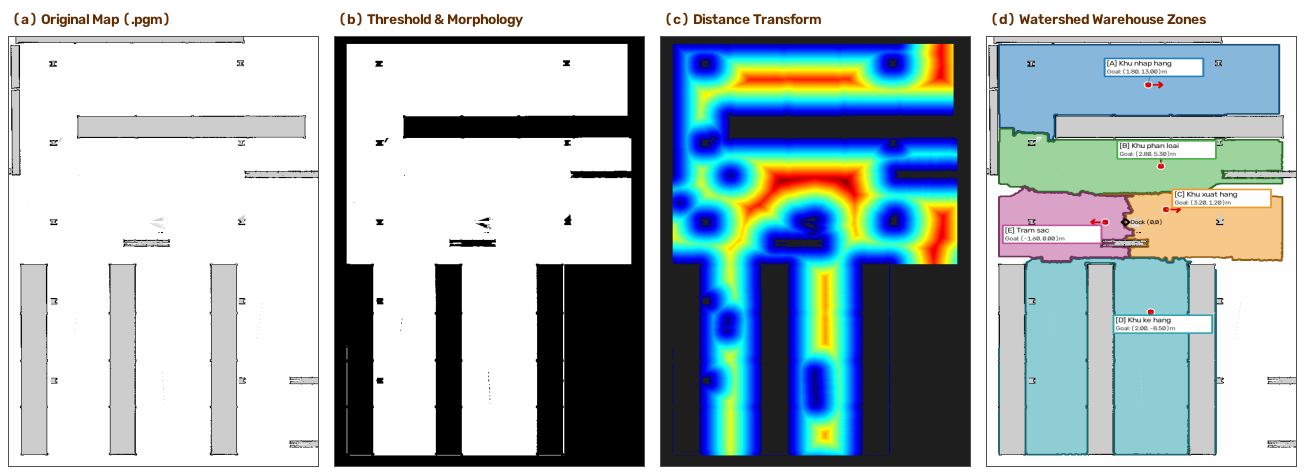
\includegraphics[width=0.92\textwidth]{figures/map_segmentation_pipeline.png}
\caption{Quy trình 4 bước phân vùng bản đồ kho vận bằng OpenCV: (1) Bản đồ gốc Occupancy Grid; (2) Phân ngưỡng nhị phân \& Lọc hình thái học; (3) Trường khoảng cách Euclid Distance Transform L2; (4) Phân vùng Watershed có hạt giống và gắn nhãn 5 phân khu chức năng}
\label{fig:pipeline_full}
\end{figure}

\begin{figure}[H]
\centering
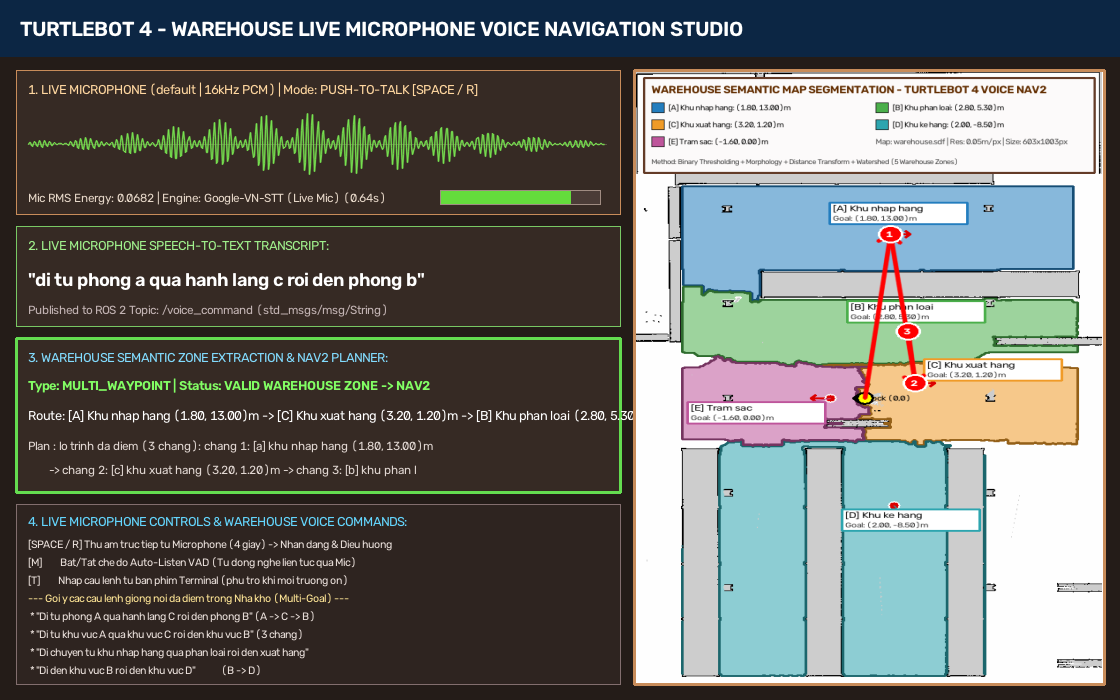
\includegraphics[width=0.88\textwidth]{figures/speech_recognition_demo.png}
\caption{Giao diện Voice Navigation Studio khi thu âm trực tiếp từ Microphone câu lệnh chuỗi liên hoàn phức tạp: hiển thị dạng sóng âm thời gian thực, bóc tách lộ trình 5 chặng liên tiếp $A \to B \to C \to D \to E$ đánh số thứ tự (1) $\to$ (2) $\to$ (3) $\to$ (4) $\to$ (5) và vẽ đường đi dự kiến kết nối toàn kho}
\label{fig:studio_full}
\end{figure}

\subsection{Kết quả kiểm thử tự động 22 kịch bản NLP toàn diện}
\begin{lstlisting}[backgroundcolor=\color{logbg}, caption={Trích xuất nhật ký kiểm thử tự động 22 kịch bản NLP trong \texttt{voice\_navigation\_node.py}}]
========================================================================
   KIEM THU BO PHAN TICH CAU LENH GIONG NOI NHA KHO (WAREHOUSE NLP)     
========================================================================
 [14] Cau lenh : "qua A qua B qua C qua D roi qua E" (Robot tai (0.35, 0.0))
      Trang thai: HOP LE | Lo trinh Waypoints: ['A', 'B', 'C', 'D', 'E']
      Chi tiet  : Lo trinh da diem (5 chang): Chang 1: [A] Khu nhap hang (1.80, 13.00)m -> Chang 2: [B] Khu phan loai (2.80, 5.30)m -> Chang 3: [C] Khu xuat hang (3.20, 1.20)m -> Chang 4: [D] Khu ke hang (2.00, -8.50)m -> Chang 5: [E] Tram sac (-1.60, 0.00)m

 [15] Cau lenh : "Di qua A, B, C, D roi den E" (Robot tai (0.35, 0.0))
      Trang thai: HOP LE | Lo trinh Waypoints: ['A', 'B', 'C', 'D', 'E']

 [16] Cau lenh : "Di tu A qua B, C, D roi ve E" (Robot tai (0.35, 0.0))
      Trang thai: HOP LE | Lo trinh Waypoints: ['A', 'B', 'C', 'D', 'E']

 [17] Cau lenh : "Di tu A qua B, C, D roi ve E" (Robot tai (1.8, 13.0) - da o A)
      Trang thai: HOP LE | Lo trinh Waypoints: ['B', 'C', 'D', 'E']
      Chi tiet  : Tu dong bo qua tram A, bat dau ngay tu tram B!

 [22] Cau lenh : "qua A qua B qua C qua Z roi qua E" (Robot tai (0.35, 0.0))
      Trang thai: TU CHOI (KHU VUC KHONG TON TAI TRONG NHA KHO) | Lo trinh: []
      Chi tiet  : Khu vuc 'Z' khong ton tai! Tu choi toan bo lo trinh, dung an toan!

========================================================================
[SELF-TEST PASSED] Tat ca 22 kich ban cau lenh giong noi nha kho chinh xac 100%!
========================================================================
\end{lstlisting}

% ==============================================================================
% MỤC 5: HƯỚNG DẪN THỰC THI & ĐƯỜNG DẪN NỘP BÀI
% ==============================================================================
\section{HƯỚNG DẪN THỰC THI \& ĐƯỜNG DẪN NỘP BÀI}

\subsection{Hướng dẫn biên dịch và khởi chạy chương trình}
\begin{lstlisting}[language=bash, caption={Các lệnh biên dịch và khởi chạy hệ thống}]
# 1. Cap nhat ma nguon tu GitHub chinh thuc va cai dat thu vien
cd /home/tuan/turtelbot4_ws/src/turtlebot4_practice4
git remote set-url origin https://github.com/Tuan404cl/Turtlebot_sim_test4.git
pip install opencv-python speechrecognition faster-whisper pyaudio sounddevice
sudo apt-get update && sudo apt-get install -y alsa-utils pulseaudio-utils

# 2. Bien dich goi turtlebot4_practice4
cd /home/tuan/turtelbot4_ws
source /opt/ros/humble/setup.bash
colcon build --symlink-install --packages-select turtlebot4_practice4
source install/setup.bash

# 3. Khoi chay toan bo he thong tich hop (01 lenh duy nhat):
./src/turtlebot4_practice4/scripts/run_voice_navigation_all.sh

# 4. Chay kiem thu rieng tung phan:
# Phan 1 - Map Segmentation:
./src/turtlebot4_practice4/scripts/run_voice_part1_segment_map.sh
# Phan 2 - Kiem tra Microphone truc tiep:
./src/turtlebot4_practice4/scripts/run_voice_part2_speech_test.sh
# Phan 3 - Kiem thu 22 kich ban NLP tu dong:
python3 /home/tuan/turtelbot4_ws/src/turtlebot4_practice4/turtlebot4_practice4/voice\_navigation\_node.py --self-test
\end{lstlisting}

\subsection{Liên kết Video Demo và GitHub Repository}
\begin{itemize}
  \item \textbf{GitHub Repository (Public):}\\
  \url{https://github.com/Tuan404cl/Turtlebot_sim_test4}
  \item \textbf{Video Demo trên Google Drive (Chế độ công khai):}\\
  \url{https://drive.google.com/drive/folders/1vl4O0C9A4C3Ed_HwHmJAeVCzwEQZulCx?usp=drive_link}
\end{itemize}

\end{document}
